\section*{The Probabilistic Framework}

Our solution is based on the concept of discrete \emph{Markov processes}, which are a type of stochastic processes. A stochastic process uses probability functions to describe how a system may pass between states. In the discrete case, the system makes discrete ``jumps'' through a discrete space of states, as opposed to the continuous case where both state transitions and state space may be continuous. A Markov process is a stochastic process that satisfies the \emph{Markov property}, which states that the system's future depends only on the current state and is independent of past states. An example of a discrete Markov process is that of throwing dice and summing the results: the throws are discrete, the sum increases by a discrete amount for each throw, and the possible sums after the next throw depends only on the current sum.

In mathematical terms, the Markov property is formulated as follows (for a discrete stochastic process):
\begin{equation}
  p\left(Z_{n+1}|Z_n, Z_{n-1}, Z_{n-2}, \dots, Z_0\right) = p\left(Z_{n+1}|Z_n\right),
\end{equation}
where $Z_n$ is the system's state after step $n$ and $p\left(Z_{n+1}|Z_n, Z_{n-1}, Z_{n-2}, \dots, Z_0\right)$ is the probability that the system will assume state $Z_{n+1}$ in the next step, given that the previous states were $Z_n, Z_{n-1}, Z_{n-2}, \dots, Z_0$.

A \emph{hidden Markov model} (HMM) describes a Markov process where one cannot measure the state $Z$ of the system directly, but rather obtains an observation $I$ of the state. This observation may not be deterministic, and so we have the probability $p(I_n|Z_n)$ that we will observe $I_n$ if the current state of the system is $Z_n$.

\subsection*{The Particle Filter}
The Particle Filter is a technique for simulating a process described by a HMM. It uses a finite set $X_n$ of $N$ hypotheses to approximate the probability function $p(Z_n)$ above. The hypotheses $X_n$ are also known as \emph{particles}, thereby the term ``particle filter''. In short terms, the particle filter does the following:

\begin{enumerate}
  \item Predicts the next state $Z_{n+1}$ by drawing samples $X_{n+1}$ from $p(Z_{n+1} | Z_n)$,
  \item resamples the hypotheses $X_{n+1}$ by drawing new samples from $p\left(I_{n+1} | x_{n+1}^i\right)$
\end{enumerate}


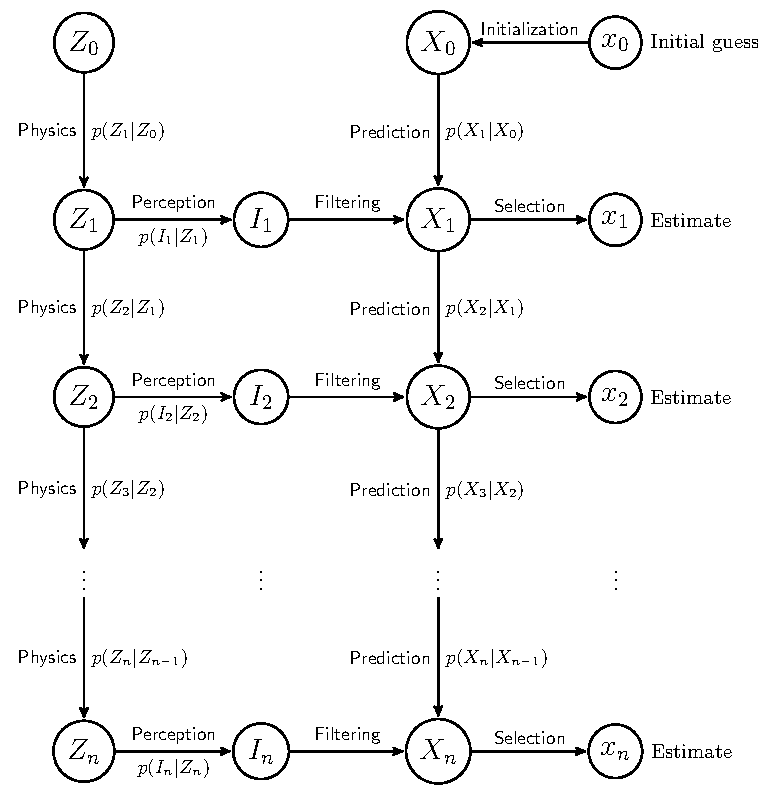
\includegraphics[width=0.3\textwidth]{figures/hmm-graph/hmm-graph.pdf}
Above is an illustration of a Particle Filter working with a Hidden Markov Model. The system assumes states $Z_0, Z_1, ...$ with probabilities $p(Z_0), p(Z_1|Z_0), \cdots$, and we obtain the observations $I_1, I_2, \cdots$ with probabilities $p(I_1|Z_1), p(I_2|Z_2), \cdots$. Parallel to this, we have a set of hypotheses $X$ for the state $Z$. The hypotheses $X_n$ of $Z_n$ are updated in the \emph{prediction} step to hypotheses $\bar{X}_{n+1}$ of $Z_{n+1}$. The image $I_{n+1}$ of the system is then used in the \emph{resampling step} to select the best hypotheses from $\bar{X}_{n+1}$, yielding the \emph{belief} $X_{n+1}$. Finally, we create a single hypothesis $x_{n+1}$ from $X_{n+1}$ that will be our estimate of the state $Z_{n+1}$.
